\documentclass{article}

\usepackage{ctex}
\usepackage{array}
\usepackage{tabularx}
\usepackage{booktabs}
\usepackage{multirow}
\usepackage{makecell}
\usepackage{graphicx}
\usepackage{amsmath}
\usepackage{lmodern}
\usepackage{amssymb}
\usepackage{amsthm}
\usepackage{listings}
\usepackage{xcolor}

\lstset{
 columns=fixed,       
 numbers=left,                                        % 在左侧显示行号
 numberstyle=\tiny\color{gray},                       % 设定行号格式
 frame=none,                                          % 不显示背景边框
 backgroundcolor=\color[RGB]{245,245,244},            % 设定背景颜色
 keywordstyle=\color[RGB]{40,40,255},                 % 设定关键字颜色
 numberstyle=\footnotesize\color{darkgray},           
 commentstyle=\it\color[RGB]{0,96,96},                % 设置代码注释的格式
 stringstyle=\rmfamily\slshape\color[RGB]{128,0,0},   % 设置字符串格式
 showstringspaces=false,                              % 不显示字符串中的空格
 breaklines=true,                                     % 对过长的代码自动换行
 language=matlab,                                     % 设置语言
}


\begin{document}
\graphicspath{{F:/School/大二下/信号与系统/project/project 1/asset}}
\title{Signal and System Project 1}
\author{HeXiang Huang}
\date{\today}
\maketitle

\section{Problem 1}
\subsection{Making Continuous-Time Pole-Zero Diagrams}
\subsubsection*{(a)}
use the following code to make the pole-zero diagram of the system
\begin{lstlisting}
%% Example
b = [1 -1];
a = [1 3 2];
zs = roots(b);
ps = roots(a);
figure(1);
subplot(2,2,1)
plot(real(zs),imag(zs),'o');
hold on;
plot(real(ps),imag(ps),'x');
title('Example')
grid;
axis([-3 3 -3 3])

%% Exercise a
% Exercise a1
a = [1 5];
b = [1 2 3];
aroot = roots(a);
broot = roots(b);
subplot(2,2,2)
plot(real(aroot),imag(aroot),'o');
hold on;
plot(real(broot),imag(broot),'x');
title('$H(s)=\frac{s+5}{s^2+2s+3}$','Interpreter','latex')
grid;
axis([-6 2 -2 2])

% Exercise a2
a = [2 5 12];
b = [1 2 10];
aroot = roots(a);
broot = roots(b);
subplot(2,2,3)
plot(real(aroot),imag(aroot),'o');
hold on;
plot(real(broot),imag(broot),'x');
title('$H(s)=\frac{2s^2+5s+12}{s^2+2s+10}$','Interpreter','latex')
grid;
axis([-2 0 -4 4])

% Exercise a3
a = [2 5 12];
b = [1 4 14 20];
aroot = roots(a);
broot = roots(b);
subplot(2,2,4)
plot(real(aroot),imag(aroot),'o');
hold on;
plot(real(broot),imag(broot),'x');
title('$H(s)=\frac{2s^2+5s+12}{(s^2+2s+10)(s+2)}$','Interpreter','latex')
grid;
axis([-3 0 -4 4])
\end{lstlisting}
Then we can get the following pole-zero diagrams
\begin{figure}[h]
    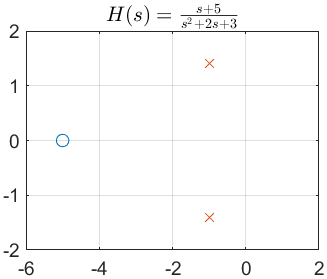
\includegraphics[width = 0.3\textwidth]{1.1.1.2.png}
    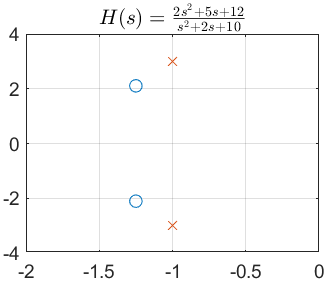
\includegraphics[width = 0.3\textwidth]{1.1.1.3.png}
    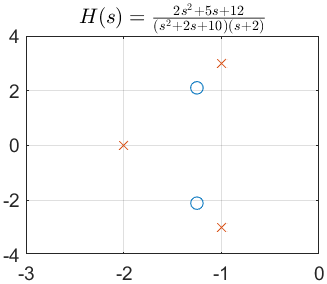
\includegraphics[width = 0.3\textwidth]{1.1.1.4.png}
\end{figure}

\subsubsection*{(b)}
A system is stable when the ROC includes the imaginary axis. 

The poles of $H(s)=\frac{s+5}{s^2+2s+3}$are $s = -1 \pm j\sqrt{2}$,
the system is stable so that the ROC is $Re(s) > -1$

The poles of $H(s) = \frac{2s^2+5s+12}{s^2+2s+10}$are $s = -1 \pm j\sqrt{3}$,
the system is stable so that the ROC is $Re(s) > -1$

The poles of $H(s)=\frac{2s^2+5s+12}{(s^2+2s+10)(s+2)}$are $s = -1 \pm j\sqrt{3}$and $s = -2$,
the system is stable so that the ROC is $Re(s) > -1$

\subsubsection*{(c)}
Do the Laplace transform of the following equations
\begin{center}
    \begin{math}
        \centering
        \frac{dy(t)}{dt} - 3y(t) = \frac{d^2x(t)}{dt^2} + 2\frac{dx(t)}{dt} + x(t)
    \end{math}
\end{center}
we can get
\begin{center}
    \begin{math}
        sY(s) - 3Y(s) = s^2X(s) + 2sX(s) + X(s)
    \end{math}
\end{center}
so that
\begin{center}
    \begin{math}
        H(s) = \frac{Y(s)}{X(s)} = \frac{s^2+2s+1}{s-3}
    \end{math}
\end{center}

The poles of $H(s) = \frac{s^2+2s+1}{s-3}$ are $s = 3$,and the zeros are $s = -1 \pm \sqrt{2}$\\

we can draw the following pole-zero diagrams
\begin{center}
    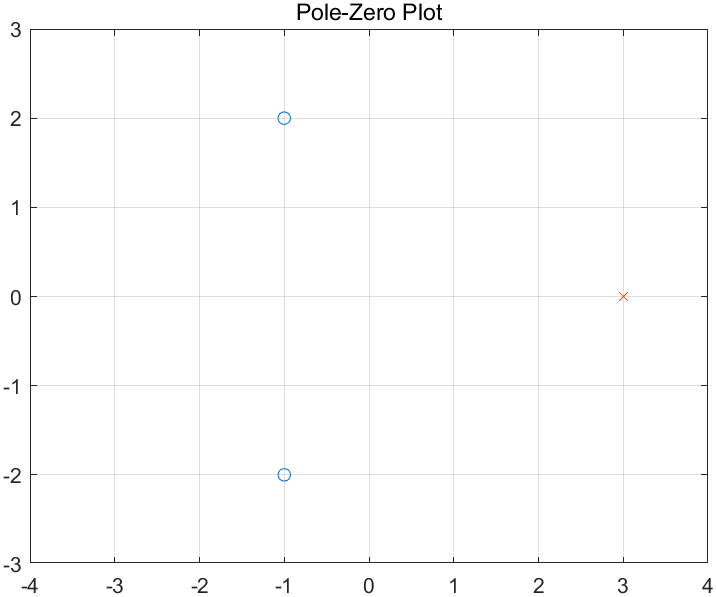
\includegraphics[width = 0.7\textwidth]{1.1.3.png}
\end{center}

\subsubsection*{(d)}
In the function pzplot,it use the function roots to find the poles and zeros of the system, and then plot the poles and zeros on the complex plane.
for every pole, if the pole is on the left side of the given point,the ROC should contain the right side of the pole, and if the pole is on the right side of the given point, the ROC should contain the left side of the pole.\\
\end{document}